\documentclass[../../main.tex]{subfiles}
\begin{document}

In this section, a similar approach is applied to the three-dimensional elastic body.


\section{A cantilever three-dimensional body}\label{sec:FEM:3D}
Consider a cantilever three-dimensional elastic body, with a rectangular cross-section.
 
\subsubsection{Reference configuration for rectangular cross-section}
Let $\{e_1,e_2,e_3\}$ be a right-handed orthonormal basis for $R^3$. Denote the elastic body as $\Omega \in R^3$ with $(0,0,0)$ the point of reference. For a rectangular cross-section, the body $\Omega$ can be described as
\begin{eqnarray*}
	\Omega = \left\{ x \in R^3 \ | \ 0 \leq x_1 \leq 1, \ -\frac{h}{2} \leq x_2 \leq \frac{h}{2} , \ -\frac{b}{2} \leq x_3 \leq \frac{b}{2}\right \}
\end{eqnarray*} \label{sym:width}
Let $\partial \Omega$ denote the boundary of the body. Divide $\partial \Omega$ into the six distinct flat surfaces as follows:

\noindent\begin{minipage}{.5\linewidth}
	\begin{eqnarray*}
		\Sigma:& \quad x_1 &= 0\\
		\Gamma_5:& \quad x_1 &= 1\\
		\Gamma_1:& \quad x_3 &= -{b}/{2} 
	\end{eqnarray*}
\end{minipage}%
\begin{minipage}{.5\linewidth}
	\begin{eqnarray*}
		\Gamma_2:& \quad x_2 &= -{h}/{2}\\
		\Gamma_3:& \quad x_3 &= {b}/{2}\\
		\Gamma_4:& \quad x_2 &= {h}/{2} 
	\end{eqnarray*}
\end{minipage}

Using this notation, the boundary conditions are similar to the two-dimensional model in Section \ref{sssec:2D_Model:RefConf}, where the body is clamped rigidly at $\Sigma$, and free-hanging on the other sides denoted by $\Gamma$.

\subsubsection{Cantilever elastic body}
Consider a three-dimensional elastic body with rectangular cross-section, rigidly clamped to a surface at attached at the side $\Sigma$ and free-hanging at all the other sides. This is Problem 3D-1 in Section \ref{ssec:3D_Model:ModelProblems}.
\FloatBarrier
\begin{figure}[h!]
	\centering
	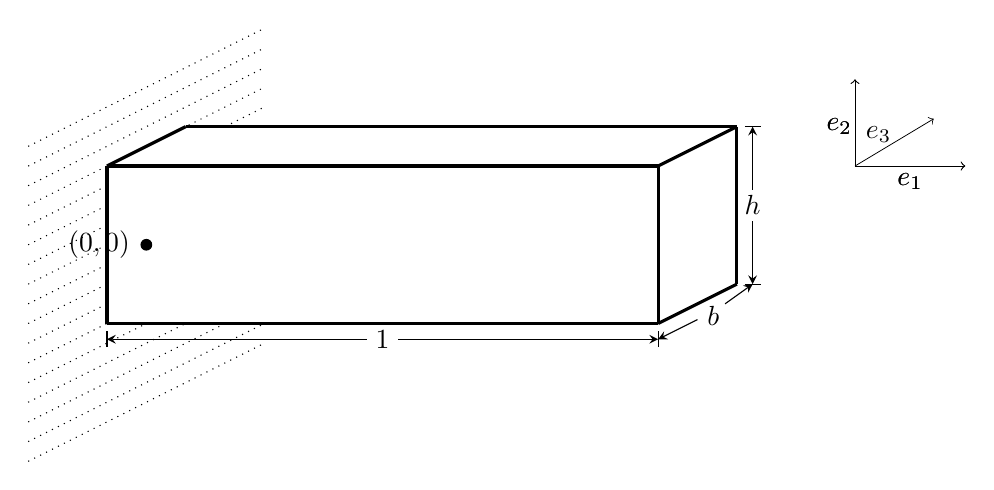
\begin{tikzpicture}
		
		\draw[line width = 0.4mm] (-0.5,1) -- (6.5,1);
		\draw[line width = 0.4mm] (-0.5,-1) -- (6.5,-1);
		\draw[line width = 0.4mm] (6.5,-1) -- (6.5,1);
		\draw[line width = 0.4mm] (-0.5,-1) -- (-0.5,1);
		
		\draw[line width = 0.4mm] (0.5,1.5) -- (7.5,1.5);
		\draw[line width = 0.4mm] (7.5,-0.5) -- (7.5,1.5);
		
		
		\draw[line width = 0.4mm] (-0.5,1) -- (0.5,1.5);
		\draw[line width = 0.4mm] (6.5,1) -- (7.5,1.5);
		\draw[line width = 0.4mm] (6.5,-1) -- (7.5,-0.5);
		
		
		
		\draw[scale=0.5, domain=-3:3, smooth, variable=\x,dotted] plot ({\x}, {0.5*\x+4});
		\draw[scale=0.5, domain=-3:3, smooth, variable=\x,dotted] plot ({\x}, {0.5*\x+3.5});
		\draw[scale=0.5, domain=-3:3, smooth, variable=\x,dotted] plot ({\x}, {0.5*\x+3});
		\draw[scale=0.5, domain=-3:3, smooth, variable=\x,dotted] plot ({\x}, {0.5*\x+2.5});
		
		\draw[scale=0.5, domain=-3:-1, smooth, variable=\x,dotted] plot ({\x}, {0.5*\x+2});
		\draw[scale=0.5, domain=2:3, smooth, variable=\x,dotted] plot ({\x}, {0.5*\x+2});
		
		\draw[scale=0.5, domain=-3:-1, smooth, variable=\x,dotted] plot ({\x}, {0.5*\x+1.5});
		\draw[scale=0.5, domain=-3:-1, smooth, variable=\x,dotted] plot ({\x}, {0.5*\x+1});
		\draw[scale=0.5, domain=-3:-1, smooth, variable=\x,dotted] plot ({\x}, {0.5*\x+0.5});
		\draw[scale=0.5, domain=-3:-1, smooth, variable=\x,dotted] plot ({\x}, {0.5*\x});
		\draw[scale=0.5, domain=-3:-1, smooth, variable=\x,dotted] plot ({\x}, {0.5*\x-0.5});
		\draw[scale=0.5, domain=-3:-1, smooth, variable=\x,dotted] plot ({\x}, {0.5*\x-1});
		\draw[scale=0.5, domain=-3:-1, smooth, variable=\x,dotted] plot ({\x}, {0.5*\x-1.5});
		\draw[scale=0.5, domain=-3:0, smooth, variable=\x,dotted] plot ({\x}, {0.5*\x-2});
		\draw[scale=0.5, domain=-3:1, smooth, variable=\x,dotted] plot ({\x}, {0.5*\x-2.5});
		\draw[scale=0.5, domain=-3:2, smooth, variable=\x,dotted] plot ({\x}, {0.5*\x-3});
		\draw[scale=0.5, domain=-3:3, smooth, variable=\x,dotted] plot ({\x}, {0.5*\x-3.5});
		\draw[scale=0.5, domain=-3:3, smooth, variable=\x,dotted] plot ({\x}, {0.5*\x-4});
		
		%\node at (6.9,1) {$b$};
		%\node at (6.65,0) {$h$};
		%\node at (3.2,-1.2) {$\ell = 1$};
		
		\draw[line width = 0.1mm,->] (9,1) -- (10,1.6);
		\draw[line width = 0.1mm,->] (9,1) -- (10.4,1);
		\draw[line width = 0.1mm,->] (9,1) -- (9,2.1);
		\node at (9.3,1.4) {$e_3$};
		\node at (9.7,0.8) {$e_1$};
		\node at (8.8,1.5) {$e_2$};
		
		\node at (7.7,0.5) {$h$};
		\draw[-stealth] (7.7,0.7) -- (7.7,1.5);
		\draw (7.6,1.5) -- (7.8,1.5);
		\draw[-stealth] (7.7,0.3) -- (7.7,-0.5);
		\draw (7.6,-0.5) -- (7.8,-0.5);
		
		\node at (3,-1.2) {$1$};
		\draw[stealth-] (-0.5,-1.2) -- (2.8,-1.2);
		\draw[stealth-] (6.5,-1.2) -- (3.2,-1.2);
		\draw (6.5,-1.3) -- (6.5,-1.1);
		\draw (-0.5,-1.3) -- (-0.5,-1.1);
		
		\node at (7.2,-0.9) {$b$};
		\draw[stealth-] (7.7,-0.5) -- (7.35,-0.75);
		\draw[stealth-] (6.5,-1.2) -- (7,-0.95);
		
		\draw[line width = 0.1mm,->] (9,1) -- (10.4,1);
		\draw[line width = 0.1mm,->] (9,1) -- (9,2.1);
		\node at (9.7,0.8) {$e_1$};
		\node at (8.8,1.5) {$e_2$};
		
		\node at (-0.6,0) {$(0,0)$};
		\node at (0,0)[circle,fill,inner sep=1.5pt]{};
		
		%\node at (-1.4,-1.3) {$(0,-\frac{h}{2},-\frac{b}{2})$};
		%\node at (-1.4,1) {$(0,\frac{h}{2},-\frac{b}{2})$};
		%\node at (0.5,1.8) {$(0,\frac{h}{2},\frac{b}{2})$};
		
		%\node at (6,-1.3) {$(1,-\frac{h}{2},-\frac{b}{2})$};
		%\node at (6.3,0.7) {$(1,\frac{h}{2},-\frac{b}{2})$};
		%\node at (7.5,1.8) {$(1,\frac{h}{2},\frac{b}{2})$};
		%\node at (8.4,-0.4) {$(1,-\frac{h}{2},\frac{b}{2})$};
		
	\end{tikzpicture}
	\caption{Cantilever Three-Dimensional Elastic Body with Rectangular Cross-Section.}
\end{figure} 
\FloatBarrier

In Section \ref{ssec:3D_Model:VariationalForm}, the variational problem for the three-dimensional cantilever model is defined by Problem 3D-1V. This general form can now be rewritten as in a model specific form using the reference configuration. For convenience, some of the results from Section \ref{sec:3D_Model} are repeated here.

\subsubsection{Problem 3D-1V}
Find a function $u$ such that for all $t>0$, $u \in T(\Omega)$ and 
\begin{align}
	c(u,\phi) = -b(u,\phi) + (Q,\phi) \label{3DB_20}
\end{align}
for all $\phi \in T(\Omega)$.\\

With the test function space
\begin{eqnarray*}
	T(\Omega) & = & \left\{ \phi \in C(\Omega) \ | \ \phi = 0 \ \textrm{ on } \ \Gamma \right\}.
\end{eqnarray*}

The bilinear forms and integral function are defined by
\begin{eqnarray}
	b(u,\phi) &=& \int_\Omega~c_1\textrm{Tr}({\cal E}\Phi)+ c_2\textrm{Tr}({\cal E})
	\textrm{Tr}(\Phi) ~dV,\\
	c(u,\phi) &=& \int_\Omega~ (\partial^2_t u) \cdot \phi~dV, \\
	(f,g) &=& \int_{\Omega} f\cdot g \ dV, \\
\end{eqnarray}
with $\displaystyle c_1 = \frac{1}{\gamma(1+\nu)}$ and $\displaystyle c_2 = \frac{\nu}{\gamma(1+\nu)(1-2\nu)}$.\\

Using the definition of the reference configuration, the constitutive equations and the bilinear form $b$ can be rewritten in the following model specific forms: 
\subsubsection*{Constitutive equations}
\begin{eqnarray*}
	\sigma_{11} & = &  \frac{1}{\gamma(1+\nu)}\partial_1 u_1 + \frac{\nu}{\gamma (1+\nu)(1-2\nu)}(\partial_1 u_1 +  \partial_2 u_2 + \partial_3 u_3)\label{3DB_3}\\
	\sigma_{22} & = &  \frac{1}{\gamma(1+\nu)}\partial_2 u_2 + \frac{\nu}{\gamma (1+\nu)(1-2\nu)}(\partial_1 u_1 +  \partial_2 u_2 + \partial_3 u_3)\label{3DB_4}\\
	\sigma_{33} & = &  \frac{1}{\gamma(1+\nu)}\partial_3 u_3 + \frac{\nu}{\gamma (1+\nu)(1-2\nu)}(\partial_1 u_1 +  \partial_2 u_2 + \partial_3 u_3)\label{3DB_5}\\
	\sigma_{23} & = &  \frac{1}{2\gamma(1+\nu)}(\partial_3 u_2 + \partial_2 u_3)\label{3DB_6}\\
	\sigma_{31} & = &  \frac{1}{2\gamma(1+\nu)}(\partial_3 u_1 + \partial_1 u_3)\label{3DB_7}\\
	\sigma_{12} & = &  \frac{1}{2\gamma(1+\nu)}(\partial_2 u_1 + \partial_1 u_2)\label{3DB_8}
\end{eqnarray*}

\subsubsection{Bilinear Form}
\begin{align*}
	b(u,\phi)  &=  \int_\Omega~c_1\textrm{Tr}({\cal E}\Phi)+ c_2\textrm{Tr}({\cal E})
	\textrm{Tr}(\Phi) ~dV \nonumber\\
	 &=  \int_{\Omega} \sigma_{11} \partial_1\phi_1 + \sigma_{12}\partial_1 \phi_2 + \sigma_{13}\partial_1 \phi_3 + \sigma_{21}\partial_2 \phi_1 + \sigma_{22}\partial_2\phi_2 + \sigma_{23}\partial_2 \phi_3 ~dV
\end{align*}

\subsection{Weak variational form}

\subsubsection{Bilinear form}
Define the inertia space $V$ as the closure of $T(\Omega)$ in $H := H^1(0,1)\times H^1(0,1)\times H^1(0,1)$. Denote $X = L^2(0,1)\times L^2(0,1)\times L^2(0,1)$. The inertia space is $W  = X$ with norm $||\cdot||_W = \sqrt{c(\cdot,\cdot)}$.

\subsubsection{Problem 3D-1W}
Find a function $u$ such that for all $t>0$, $u(t) \in V$ and $u''(t) \in W$, satisfying the following equation
\begin{eqnarray}
	c(u,v) + b(u,v) & = & (Q,v) \ \ \ \textrm{ for each } v \in V.
\end{eqnarray}

See Chapter 2 for the existence theory.

\subsection{Galerkin approximation}
As mentioned in the previous section, Section \ref{2d_FEM_G}, the body $\Omega$ needs to be descritised. For this three-dimensional body, three-dimensional elements shapes are required. The elements used in this dissertation are rectangular prismatic elements. These elements are also known as `brick-shaped' elements and is described in \cite{Wu06}. This shape of element is a natural choice for a three-dimensional elastic body with a rectangular cross-section.

Divide the reference configuration $\Omega$ into a grid of rectangular prismatic elements, such that there are $n = n_1 \times n_2 \times n_3$ nodes.

Define a set of $n$-dimensional linear independent basis functions. For the three-dimensional model, the basis functions can be defined by the set
\begin{eqnarray*}
 B = \{\langle\phi_1, 0 , 0\rangle, \langle\phi_2, 0, 0\rangle,...,\langle\phi_{n}, 0, 0 \rangle,\\
	\langle 0,\phi_1 ,0 \rangle,\langle 0 ,\phi_2,0\rangle,...,\langle 0,\phi_{n},0\rangle,\\
	\langle 0,0,\phi_1 \rangle,\langle 0,0,\phi_2\rangle,...,\langle 0,0,\phi_{n}\rangle \}.
\end{eqnarray*}

For this three-dimensional model, piecewise Hermite tri-cubic basis functions are used. Although this is more complex than using piecwise tri-linear basis functions, as mentioned in Section \ref{2d_FEM_G}, the tri-cubic basis functions ensure faster convergence and also the derivatives of the solutions.

Recall that the admissible basis functions, are all the basis functions that satisfies all the conditions of the test function space $T(\Omega)$. Denote the admissible basis functions by $\delta_j$, with each $\delta_j$ a unique element of $B$. The set of admissible basis functions can then be expressed as $A = \left\{\delta_1, \delta_2,... , \delta_k\right\}$ with $k \leq 3n$.

Define the space
\begin{eqnarray*}
	S^h & = & \textrm{span}\left\{\delta_i \ | \ i = 1,2,...,k \right\}
\end{eqnarray*}

For each function $u^h \in S^h$, $u^h$ can be expressed as
\begin{eqnarray*}
	u^h = \sum_{i = 1}^{k} u_i(t) \delta_{i}(x)
\end{eqnarray*}

Substituting $u^h$ into Problem 3D-1V, results in the following Galerkin approximation, denoted by Problem 3D-1G.

\subsubsection{Problem 3D-1G}
Find a function $u^h$ such that for all $t>0$, $u^h \in S^h$ and
\begin{eqnarray*}
	(u^h, \phi_i) & = & -b(u^h,\phi_i) + (Q^I \cdot \phi_i)
\end{eqnarray*} for $i = 1,2,...,k$. $Q^I$ is a scalar vector obtained after interpolating the function $Q$ over the rectangular grid $\Omega$, i.e. $Q^I_{i,j, h} = Q(x_i,x_j, x_h)$ for $i = 1,2,...,n_1$, $j = 1,2,...,n_2$ and $h = 1,2,...,n_3$.

\subsection{System of ordinary differential equations}\label{3d_fem_g}
Consider the following standard Finite Element Method matrices.

\subsubsection{FEM matrices}
\noindent\begin{minipage}{.5\linewidth}
	\begin{eqnarray*}
		\mathbf{M}_{ij} & = & \int_{\Omega} \phi_j \phi_i \ dV \ \\
		{K_{11}}_{ij} & = & \int_{\Omega} \partial_1\phi_j \partial_1\phi_i \ dV \  \\
		{K_{12}}_{ij} & = & \int_{\Omega} \partial_1\phi_j \partial_2\phi_i \ dV \ \\
		{K_{13}}_{ij} & = & \int_{\Omega} \partial_1\phi_j \partial_3\phi_i \ dV \ 
	\end{eqnarray*}
\end{minipage}%
\begin{minipage}{.5\linewidth}
	\begin{eqnarray*}
		{K_{22}}_{ij} & = & \int_{\Omega} \partial_2\phi_j \partial_2\phi_i \ dV \  \\
		{K_{23}}_{ij} & = & \int_{\Omega} \partial_2\phi_j \partial_3\phi_i \ dV \ \\
		{K_{33}}_{ij} & = & \int_{\Omega} \partial_3\phi_j \partial_3\phi_i \ dV \ \\
	\end{eqnarray*}
\end{minipage}

for $i,j = 1,2,...,k.$\\

And

\begin{eqnarray*}
	\mathbf{M_f}_{ij} & = & \int_{\Omega} \phi_j \phi_i \ dV
\end{eqnarray*}
for $i = 1,2,...,k$ and for $j = 1,2,...,3n.$\\

The remaining matrices can be defined as
\begin{eqnarray*}
	{K_{21}} & = & {K_{12}}^{T},\\
	{K_{31}} & = & {K_{13}}^{T}, \\
	{K_{32}} & = & {K_{23}}^{T}. \\
\end{eqnarray*}

Define the following matrices:\\
\noindent\begin{minipage}{.5\linewidth}
	\begin{eqnarray*}
		\mathbf{K11} & = & \left(C_1 + C_2 \right) K_{11} + C_3 K_{22} + C_3 K_{33}\\
		\mathbf{K12} & = & C_3 K_{12} + C_2 K_{21}\\
		\mathbf{K13} & = & C_3 K_{13} + C_2 K_{31}\\
		\mathbf{K21} & = & C_3 K_{21} + C_2 K_{12}\\
		\mathbf{K22} & = & \left(C_1 + C_2 \right) K_{22} + C_3 K_{11} + C_3 K_{33}
	\end{eqnarray*}
\end{minipage}%
\begin{minipage}{0.8\linewidth}
	\begin{eqnarray*}
		\mathbf{K23} & = & C_3 K_{23} + C_2 K_{32}\\
		\mathbf{K31} & = & C_3 K_{31} + C_2 K_{13}\\
		\mathbf{K32} & = & C_3 K_{32} + C_2 K_{23}\\
		\mathbf{K33} & = & \left(C_1 + C_3 \right) K_{33} + C_3 K_{11} + C_3 K_{22}
	\end{eqnarray*}
\end{minipage}\\

with $C_1 = \frac{1}{\gamma(1+\nu)}$, $C_2 =  \frac{\nu}{\gamma (1+\nu)(1-2\nu)}$ and $C_3 =  \frac{1}{2\gamma(1-2\nu)}$.\\

Using the standard FEM matrices and the matrices $K11$ to $K33$, the following concatenated matrices are defined:\\


\begin{eqnarray}
	\begin{aligned}
		K = 
		\begin{bmatrix}
			\mathbf{K11} & \mathbf{K12} & \mathbf{K13}\\
			\mathbf{K21} & \mathbf{K22} & \mathbf{K23}\\
			\mathbf{K31} & \mathbf{K32} & \mathbf{K33}
		\end{bmatrix}
	\end{aligned}
	\ \ \ \ \ \ \ \ \
	\begin{aligned}
		M  = 
		\begin{bmatrix}
			\mathbf{M} & {O} & {O}\\
			{O} & \mathbf{M} & {O}\\
			{O} & {O} & \mathbf{M}
		\end{bmatrix}
	\end{aligned}\label{eq:3DFEM:K+M}
\end{eqnarray}



\begin{eqnarray}
	M_f & = &
	\begin{bmatrix}
		\mathbf{M_f} & {O_f} & {O_f}\\
		{O_f} & \mathbf{M_f} & {O_f}\\
		{O_f} & {O_f} & \mathbf{M_f}
	\end{bmatrix}\label{eq:3DFEM:M}
\end{eqnarray}
The matrices ${O}$ and ${O_f}$ are the zero matrices of the same size as $\mathbf{M}$ and $\mathbf{M_f}$ respectively.\\

Using \eqref{eq:3DFEM:K+M} and \eqref{eq:3DFEM:M}, Problem 3D-1G is rewritten as a system of ordinary differential equations. This system is referred to as Problem 3D-1ODE

\subsubsection{Problem 3D-1ODE}
Find a function $\bar{u} \in S^h$ such that
\begin{eqnarray}
	M\ddot{\bar{u}} & = & K\bar{u} + M_{f}Q^I. \label{3D_M}
\end{eqnarray} With $\bar{u}$ in the form $\bar{u} = \langle \partial^i_1u, \ \partial^j_2u, \ \partial^k_3u \rangle$ for $i,j,k = 0,1,2,3$.

\subsection{Eigenvalue problem}
The derivation and form of the eigenvalue problem for the three-dimensional elastic body is similar to the two-dimensional model given in Section \ref{2dFEM_EP}.

\subsubsection{Problem 3D-1E}\label{3dFEM_EP}
Find a real number $\lambda$ and a function $\bar{u} \in S^h$ such that
\begin{eqnarray}
	M\lambda{\bar{u}} & = & K\bar{u}.
\end{eqnarray}

\end{document}

Consider a set of $n$ linear independent three-dimensional scalar valued functions $\delta_i$. In this dissertation, these functions are piecewise Hermite tri-cubic basis functions (an extension of Hermite cubics from the two-dimensional model into three-dimensions). The functions $\delta_i$ satisfying the conditions of the test function space $T(\Omega)$ are called the admissible basis functions. Since there are a finite number if admissible basis functions, they can be numbered $\delta_1, \delta_2,...,\delta_k$.\\

Let $S^h$ be a $3k$-dimensional subset of $T(\Omega)$ where
\begin{eqnarray*}
	S^h & = & \textrm{span}(\left\{\langle \delta_i, 0,  0\rangle \ | \ i = 1,2,...,p \right\} \cup \left\{\langle 0, \delta_i, 0\rangle \ | \ i = 1,2,...,p \right\}\\
	&& \quad \quad \quad \quad \quad  \cup \left\{\langle 0, 0, \delta_i\rangle \ | \ i = 1,2,...,p \right\} ).
\end{eqnarray*}

The body $\Omega$ is divided into an $n_1 \times n_2 \times n_3$ grid consisting of rectangular prism shaped elements. This is described as ``bricked-shaped'' elements in [WuXX]. Let $x^*_i = \langle x_1,x_2,x_3\rangle \in \Omega$ where $\delta_i(x_1,x_2,x_3) = 1$. Define $\bar{x} = \langle x_1^*,x_2^*,...,x_k^* \rangle$.  For each solution $u$ of Problem 3D-1V let $u^h$ denote the projection of $u$ into the finite dimensional space $S^h$. Each function $u^h=\langle u_1^h,u_2^h,u_3^h\rangle$ in S$^h$ can be expressed as
\begin{eqnarray*}
	w_1^h(\bar{x},t) = \sum_{i = 1}^{p} w_{1}(x_i^*,t) \delta_{i}(\bar{x}), \ \ \ w_2^h(\bar{x},t) = \sum_{i = 1}^{p} w_{2}(x_i^*,t) \delta_{i}(\bar{x})\\
	\ \ \   \textrm{ and }  w_3^h(\bar{x},t) = \sum_{i = 1}^{p} w_{3}(x_i^*,t) \delta_{i}(\bar{x}).
\end{eqnarray*}

Then Problem 3D-1V can be rewritten into a Galerkin Approximation, denoted by Problem 3D-1G
